
\chapter{Shape Analysis}
Pointers and heap-allocated storage are features of all modern imperative programming languages.
They are among the most
complicated features of imperative programming language:
updating pointer variables (or pointer-fields of records) may have large side effects.
For example, dereferencing a pointer that has been freed will lead to segmentation fault in a C or C++ program.
Such side effects also make program analysis harder, because they make it
difficult to compute aliasing relationships among different pointers in a program. Aliasing arises when the same memory location can be accessed using different names.
For instance, consider the instruction statement $\tt x.f := y$ in an imperative language, where $\tt x$ and $\tt y$ are pointer variables. Its effect is to assign the value of the pointer $\tt y$ to the cell pointed to by $\tt x.f$. In order to update aliasing information of $\tt y$. We have to require information about all the cell pointed by $\tt x.f$ which is not an easy task.
%\bjcom{The last two sentences do not make sense (e.g., x.f points to exactly one
%  cell, so what means ``all cells''?). Make a new try}

In verification and program analysis, it is a problem to deduce and describe  how the heap-allocated memory is organized. E.g., program invariants must often describe how the heap-allocated memory is structured in order to infer the effects of statements that dereference pointer fields. This is the topic of ``shape analysis''.


%\bjcom{First sentence must be rewritten}
\section{Previous Approaches} 

Shape analysis is a generic term denoting static
program-analysis techniques that attempt to discover and verify properties of the heap contents in (usually imperative) programs. The shape analysis problem becomes more challenging in concurrent programs that manipulate pointers and dynamically allocated objects, which are usually complicated. 
In concurrent programs, different threads interact in complex ways, which are difficult to foresee in the analysis. Several approaches for representing the possible structures of the heap have been proposed.
\begin{figure}
\center 
\begin{tikzpicture}[]


\node[rounded corners,draw,name=cell1,minimum width=24pt, minimum height=20pt]{};
\node[minimum width=8pt, minimum height=10pt,anchor=north west,font=\tiny,inner sep=0pt,name=d1] at (cell1.north west){$\mkadata0$};
\node[minimum width=8pt, minimum height=10pt,anchor=south west,font=\tiny,inner sep=0pt,scale=0.8] at ($(cell1.south west)+(0.5pt,1pt)$){{--$\infty$}};
\node[draw,minimum width=8pt, minimum height=10pt,anchor=north,font=\tiny,inner sep=0pt]at (cell1.north){\cross};
\node[draw,minimum width=8pt, minimum height=10pt,anchor=south,font=\tiny,inner sep=0pt]at (cell1.south){\cross};
\node[name=succ1,circle,fill,minimum size=3pt,inner sep=0pt,outer sep=0pt] at ($(cell1.east)+(-4pt,0pt)$) {};
\node[anchor=north,font=\tiny,align=center] at ($(cell1.south)+(0pt,2pt)$) {{\tt head}};

\node[rounded corners,draw,name=cell2,minimum width=24pt, minimum height=20pt,anchor=west]
at ($(cell1.east)+(10pt,0pt)$){};
\node[minimum width=8pt, minimum height=10pt,anchor=north west,font=\tiny,inner sep=0pt,name=d2] at (cell2.north west){$\mkadata0$};
\node[minimum width=8pt, minimum height=10pt,anchor=south west,font=\tiny,inner sep=0pt] at (cell2.south west){$3$};
\node[draw,minimum width=8pt, minimum height=10pt,anchor=north,font=\tiny,inner sep=0pt]at (cell2.north){\cross};
\node[draw,minimum width=8pt, minimum height=10pt,anchor=south,font=\tiny,inner sep=0pt]at (cell2.south){\tick};
\node[name=succ2,circle,fill,minimum size=3pt,inner sep=0pt,outer sep=0pt] at ($(cell2.east)+(-4pt,0pt)$) {};
\draw[->] (succ1) -- (cell2);
\draw[->,dotted,line width=1pt,color=blue,out=90,in=120] ($(d1.north)+(0pt,0pt)$) to ($(d2.north west)+(1pt,-1pt)$);
\node[anchor=north,font=\tiny,align=center] at ($(cell2.south)+(0pt,2pt)$) {$\tuple{\thread_{\tt 1},{\tt p}}$\\$\tuple{\thread_{\tt 2},{\tt p}}$};



\node[rounded corners,draw,name=cell3,minimum width=24pt, minimum height=20pt,anchor=west]
at ($(cell2.east)+(10pt,20pt)$){};
\node[minimum width=8pt, minimum height=10pt,anchor=north west,font=\tiny,inner sep=0pt,name=d3] at (cell3.north west){$\mkadata1$};
\node[minimum width=8pt, minimum height=10pt,anchor=south west,font=\tiny,inner sep=0pt,name=d3a] at (cell3.south west){$4$};
\node[draw,minimum width=8pt, minimum height=10pt,anchor=north,font=\tiny,inner sep=0pt]at (cell3.north){\cross};
\node[draw,minimum width=8pt, minimum height=10pt,anchor=south,font=\tiny,inner sep=0pt]at (cell3.south){\cross};
\node[name=succ3,circle,fill,minimum size=3pt,inner sep=0pt,outer sep=0pt] at ($(cell3.east)+(-4pt,0pt)$) {};
\draw[->,out=0,in=180] (succ2) to (cell3.west);
\draw[->,dotted,line width=1pt,color=blue,out=60,in=180] ($(d2.north)+(3pt,0pt)$) to ($(d3.west)$);
\node[anchor=south,font=\tiny,align=center] at ($(cell3.north)+(0pt,-2pt)$) {$\tuple{\thread_{\tt 2},{\tt n}}$};



\node[rounded corners,draw,name=cell4,minimum width=24pt, minimum height=20pt,anchor=west]
at ($(cell3.east)+(10pt,-20pt)$){};
\node[minimum width=8pt, minimum height=10pt,anchor=north west,font=\tiny,inner sep=0pt,name=d4] at (cell4.north west){$\mkadata0$};
\node[minimum width=8pt, minimum height=10pt,anchor=south west,font=\tiny,inner sep=0pt,name=d4a] at (cell4.south west){$6$};
\node[draw,minimum width=8pt, minimum height=10pt,anchor=north,font=\tiny,inner sep=0pt]at (cell4.north){\cross};
\node[draw,minimum width=8pt, minimum height=10pt,anchor=south,font=\tiny,inner sep=0pt]at (cell4.south){\tick};
\node[name=succ4,circle,fill,minimum size=3pt,inner sep=0pt,outer sep=0pt] at ($(cell4.east)+(-4pt,0pt)$) {};
\draw[->,out=0,in=180] (succ3) to  ($(cell4.west)+(0pt,6pt)$);
\node[anchor=south,font=\tiny,align=center] at ($(cell4.north)+(0pt,-2pt)$) {$\tuple{\thread_{\tt 2},{\tt c}}$};


\node[rounded corners,draw,name=cell5,minimum width=24pt, minimum height=20pt,anchor=west]
at ($(cell4.east)+(10pt,0pt)$){};
\node[minimum width=8pt, minimum height=10pt,anchor=north west,font=\tiny,inner sep=0pt,name=d5] at (cell5.north west){$\mkadata0$};
\node[minimum width=8pt, minimum height=10pt,anchor=south west,font=\tiny,inner sep=0pt,name=d5a] at (cell5.south west){$9$};
\node[draw,minimum width=8pt, minimum height=10pt,anchor=north,font=\tiny,inner sep=0pt]at (cell5.north){\cross};
\node[draw,minimum width=8pt, minimum height=10pt,anchor=south,font=\tiny,inner sep=0pt]at (cell5.south){\cross};
\node[name=succ5,circle,fill,minimum size=3pt,inner sep=0pt,outer sep=0pt] at ($(cell5.east)+(-4pt,0pt)$) {};
\draw[->] (succ4) -- (cell5);
\draw[->,dotted,line width=1pt,color=blue,out=270,in=270] ($(d4a.south)+(0pt,0pt)$) to ($(d5a.south)+(-3pt,1pt)$);
\node[anchor=south,font=\tiny,align=center] at ($(cell5.north)+(0pt,-2pt)$) {$\tuple{\thread_{\tt 3},{\tt c}}$};


\node[rounded corners,draw,name=cell6,minimum width=24pt, minimum height=20pt,anchor=west,name=cell6]
at ($(cell5.east)+(10pt,0pt)$){};
\node[minimum width=8pt, minimum height=10pt,anchor=north west,font=\tiny,inner sep=0pt,name=d6] at (cell6.north west){$\mkadata0$};
\node[minimum width=8pt, minimum height=10pt,anchor=south west,font=\tiny,inner sep=0pt,scale=0.8,name=d6a] at ($(cell6.south west)+(1pt,1pt)$){$\infty$};
\node[draw,minimum width=8pt, minimum height=10pt,anchor=north,font=\tiny,inner sep=0pt]at (cell6.north){\cross};
\node[draw,minimum width=8pt, minimum height=10pt,anchor=south,font=\tiny,inner sep=0pt]at (cell6.south){\cross};
\draw ($(cell6.north east)+(-1pt,-2pt)$) -- ($(cell6.south east)+(-8pt,0pt)$);
\draw ($(cell6.north east)+(-8pt,0pt)$) -- ($(cell6.south east)+(-1pt,2pt)$);
\draw[->] (succ5) -- (cell6);
\draw[->,dotted,line width=1pt,color=blue,out=270,in=270] ($(d5a.south)+(3pt,0pt)$) to ($(d6a.south)+(0pt,-1pt)$);
\node[anchor=south,font=\tiny,align=center] at ($(cell6.north)+(0pt,-2pt)$) {{\tt tail}};

\node[rounded corners,draw,name=cell7,minimum width=24pt, minimum height=20pt,anchor=west]
at ($(cell2.east)+(7pt,-20pt)$){};
\node[minimum width=8pt, minimum height=10pt,anchor=north west,font=\tiny,inner sep=0pt,name=d7] at (cell7.north west){$\mkadata1$};
\node[minimum width=8pt, minimum height=10pt,anchor=south west,font=\tiny,inner sep=0pt] at (cell7.south west){$4$};
\node[draw,minimum width=8pt, minimum height=10pt,anchor=north,font=\tiny,inner sep=0pt]at (cell7.north){\tick};
\node[draw,minimum width=8pt, minimum height=10pt,anchor=south,font=\tiny,inner sep=0pt]at (cell7.south){\tick};
\node[name=succ7,circle,fill,minimum size=3pt,inner sep=0pt,outer sep=0pt] at ($(cell7.east)+(-4pt,0pt)$) {};
\draw[->,out=0,in=180] (succ7) to ($(cell4.west)+(0pt,-6pt)$);
\draw[<->,dotted,line width=1pt,color=blue,out=270,in=90] ($(d3a.south)$) to ($(d7.north)+(-2pt,0pt)$);
\draw[->,dotted,line width=1pt,color=blue,out=90,in=180] ($(d7.north)+(2pt,0pt)$) to ($(cell4.west)$);
\node[anchor=north,font=\tiny,align=center] at ($(cell7.south)+(0pt,2pt)$) {$\tuple{\thread_{\tt 1},{\tt c}}$};

\end{tikzpicture}
\caption{A heap configuration of the {\tt Lazy Set} Algorithm. The abstract data values, 
and the dotted arrows represent performing data abstraction.
There are three active threads $\thread_1$, $\thread_2$, and $\thread_3$,
running the methods ${\tt rmv}(4)$, ${\tt add}(4)$, and ${\tt ctn}(9)$ respectively.
%
The symbols \tick and \cross represent the Boolean values {\tt true} and {\tt false}.}
\label{lazy:list:heap:fig}
\end{figure}
%

TVLA (Three-Valued Logic Analysis) \cite{SagivRW02} is one of the first and one of the most popular shape analysis
methods. It is based on a three-valued first-order predicate logic with transitive closure. Intuitively, concrete heap structure is represented by a finite set of abstract summary cells, each of them representing a set of concrete cells. Summary cells are obtained by merging several heap cells that agree on the values of a chosen set of unary abstraction predicates.  %\bjcom{I think the explanation of summary cells should be improved to be understandable. You might consider putting a small illustration of what is a summary cell. }
A unique important aspect of TVLA is that it automatically generates the abstract transformers from the concrete semantics; these transformers are guaranteed to be sound, and precise enough to verify wide ranges of applications. However, it cannot fully automatically handle all programs, and that one may have to extend it by appropriate predicates etc. Its the synthesis of appropriate predicates that are able to express the invariants in the program. This problem is even more difficult with complicated heap structures such as skip-lists, trees, or arrays of lists.  

There are several other approaches
 based on the use of logics to present heap configurations. The logics can be separation logic \cite{John:SL, Stephen:SL,JoshCris:SL,Hongseok:SL,Kamil:SL,Chin:SL,Quang:SL, Ruzica:SL, Constrantin:SL}, monadic second-order
 % \bjcom{check how to separate or conjoin ``second'' ``order''}
 logic \cite{Ander:ML, Jakob:ML,Madhusudan:ML} and others \cite{Shmuel:Shape, Karen:Shape}. Among these works, the works based on separation logic are
 %such as \cite{JoshCris:SL,Hongseok:SL, Quang:SL} 
  more efficient than the others. 
  %\bjcom{The preceding sentence had no information. You can improve it} 
  The reason for that is that their approaches effectively decompose the heap into disjoint components and treat them independently. However, most of the techniques based on separation logic are either specialised for some particular data structure, or they need to be provided inductive definitions of the data structures. In addition, their entailment checking procedures are either for specific class of data structures or based on folding/unfolding inductive predicates in the formulae and trying to obtain a syntactic proof of the entailment. 

 
 This issue can be fixed addressed by automata-based techniques using the generality of the automata-based representation such as techniques using tree automata. Finite tree automata, for instance, have been shown to provide a good balance between efficiency and expressiveness. The work \cite{Ahmed:TreeAutomata} uses a finite tree automaton to describe a set of tree parts and represent non-tree edges of heaps by using regular “routing” expressions. Finite tree transducers
are used to compute set of reachable configurations, and symbolic configuration is abstracted
collapsing certain states of the automata. The refinement technique called counterexample-guided
abstraction refinement (CEGAR) technique is used during the run of the analysis. This technique
is fully automatically and can handle complex data structures such as binary trees with linked
leaves. However, it suffers from the inefficiency and it also can not handle concurrent programs.
%\bjcom{The preceding paragraph was interesting, but too hard to follow. Try to
%  explain in a more understandable way}

The problem of inefficiently of the previous technique can be solved by the approach based on forest automata \cite{foresterfull}. In such representation, a heap is split in a canonical way into several tree components whose roots are the so-called cut-points. Cut-points are cells which are pointed to by either program variables or having several incoming edges. The tree components can refer to the roots of each other, and hence they are “separated” much like heaps described by formulae joined by the separating conjunction in separation logic \cite{John:SL}. Using this decomposition, sets of heaps with a bounded number of cut-points can then be represented by so called forest automata (FA). Each of the tree
automata within the tuple accepts trees whose leaves may refer back to the
roots of any of these trees. A forest automaton then represents exactly the set
of heaps that may be obtained by taking a single tree from the language of each
of the component tree automata and by gluing the roots of the trees with the
leaves referring to them. %\bjcom{Previous sentences was a good explanation. Now
  %introduce the example, and discuss nested FAs only later}
 Moreover, they allow alphabets of FA to contain nested FA, leading to a hierarchical encoding of heaps, allowing us to represent even sets of heaps with an unbounded number of cut-points (e.g., sets of DLL, skiplist). \input FA
Let us take an example of how to split a heap into small tree components. Figure \ref{forestautomata} shows five tree components obtained by splitting the heap in figure \ref{lazy:list:heap:fig}. These components are named as 1,2,3,4 and 5 from left to right. Each root of a tree component is a cut-point in the heap in figure \ref{lazy:list:heap:fig}. These cut-points are cells pointed to by variables $\tt head$, $\tt tail$,  $\tt p$,  $\tt c$ and the cell which has two incoming pointers. In each tree component, the red node show which  tree component it refers. For instance, the tree component 1 refers to tree component 2, and both tree components 2 and 3 refer to tree component 4.
%\bjcom{The number of pictures is buggy in preceding paragraph.
%Check \url{http://www.terminally-incoherent.com/blog/2007/04/14/latex-fixing-wrong-figure-numbers/}}

This forest automata approach is fully automatic and able to verify various classes of data structures, including complicated structures such as trees and skip-lists with bounded number of levels. 
However, the approach can not verify properties related to data values of heap cells such as sortedness in the lazy set algorithm. Therefore, in this thesis, we extend their work to verify data properties. 
%bjcom{This paragraph can be extended so that it mentions the challenges that
%  you will address in papers I, II, and III: You can start from the FA approach
%  and mention what it cannot do. Thereafter, you will have sections for each
%  challenge in ``Our Approaches''. For instance, you can focus on
%data in paper I, concurrency in Paper II, and non-SLL structures in paper III}

The last approach that we will mention is based on graph grammars describing heap graphs \cite{Jonathan:Shape, Jonathan:Grammars}.  The approach is to model heap states hypergraphs, and represent both pointer operations and abstraction mappings by hypergraph transformations. The presented approaches differ in their degree of specialisation for a particular class of data structures, their efficiency, and their level of dependence on user assistance (such as definition of loop invariants or inductive predicates for the considered data structures).
  
\section{Our Approaches}
%\bjcom{Use the present tense}
In this thesis, we propose three approaches for heap abstractions. In paper I, we propose a novel approach of extending the forest automata approach \cite{foresterfull} by expressing relationships between data elements associated with cells of the heap %\bjcom{Did you explain the term ``heap graph''?} 
by two classes of constraints.
%representing sets of heaps via tree automata (TA). In our representation, a heap is split in a canonical way into several tree components whose roots are the so-called cut-points. Cut-points are nodes pointed to by program variables or having several incoming edges. The tree components can refer to the roots of each other, and hence they are “separated” much like heaps described by formulae joined by the separating conjunction in separation logic [15]. Using this decomposition, sets of heaps with a bounded number of cut-points are then represented by the so called forest automata (FA) that are basically tuples of TA accepting tuples of trees whose leaves can refer back to the roots of the trees. Moreover, we allow alphabets of FA to contain nested FA, leading to a hierarchical encoding of heaps, allowing us to represent even sets of heaps with an unbounded number of cut-points (e.g., sets of DLL, skiplist).
%\bjcom{Separate the text so that previous FA work is in previous section (as
%  you have now). In this section, you describe how you extend the FA approach}
\input TA

 %\bjcom{You can be more clear by putting bullets here: e.g., one for local and one for global}
 \begin{itemize}
 	\item Local data constraints are associated with transitions of each TA and capture relationships between data of neighboring cells in a heap; they can be used, e.g., to represent ordering internal to data structures such as sorted linked lists and binary search trees.
 	\item Global data constraints are associated with states of TA and capture relationships between data in distant parts of the heap. Intuitively, a global data constraint between two TAs captures the data relationship between cells of two heaps accepted by these two TAs. 
 %\bjcom{At this point, the text needs an illustration. Only thereafter you explain what the approach can accomplish}
 \end{itemize}
Figure \ref{figure:forest} shows an example of how to represent a heap in \ref{lazy:list:heap:fig} by a set of tree automata with added data constraints. In the figure, the local data constraints are located along the solid arrows between cells, whereas global constraints are located along the blue arrows. The global constraint $\tt \prec_{aa}$ means that data values of all cells in the left hand side are smaller than data values of all cells in the right hand side. The local constraint $\tt \prec_{rr}$ means that left hand side cell is smaller than data value of the cell in the right hand side. For instance, in tree component 1, the data value of the cell pointed to by $\tt head$ is smaller than its successor whose data value is 4, and data values of all cells in tree component 1 are smaller than data values of all cells in tree component 2. We just show here small examples of data constraints, the detail about different types of constraints can be found in paper I.    

This approach was applied to verification of sequential heap manipulation programs. This approach is general and able to verify properties of many types of sequential programs without any manual step. However, due to the complexity of tree automata operations, this approach is not optimal to handle concurrent programs where a large number of states and computation are needed. 
%\bjcom{Here, a new (sub)section is needed}
In order to verify concurrent data structures with unbounded number of threads, thread-modular is a promising approach for this challenge. Its high efficiency is achieved by
abstracting the interaction between threads. The approach verifies a concurrent data structure by generating an invariant that correlates the global state with the local state of an
arbitrary thread. In other words, it only keep track of the shape viewed by one thread, while abstracting away all the other threads. The thread-modular
approach includes a step where it takes the information about one thread and
intersect it with the information from another thread, in order to take into account the interference of all the other threads on the first thread. Forest automata approach is not suitable for this thread-modular. The reason is that computing intersection between FAs is not efficient in concurrent systems where the number of FAs is huge. 

Therefore, in paper II, we adapt FA to the new setting by providing a symbolic encoding of the heap structure, that is less precise than the forest automata approach in paper I. However it is precise enough to allow the verification of the concurrent data structures, and efficient enough to make the verification procedure feasible in practice.
% \bjcom{The text that introduce paper II does not give a good picture. First of all, you must introduce the thread-modular
%  approach, and illustrate it, i.e., one challenge is to cope with concurrency.
%Thereafter, you can say that you need to adapt FA to the new setting.
%You can say that your approach is now specialized for SLLs. You can introduce it by saying that TAs are replaced by ``heap segments''. (is it true that a heap
%segment can be characterized by a TA with data constraints?).
%Then you can explain whether cut points are now the same as for FAs or
%whether they are different.}
The main idea of the abstraction is to have a more precise description of the parts of the heap that are visible (reachable) from global variables, and to make a succinct representation of the parts that are local to the threads. Intuitively, a heap segment can be characterized by a TA with data constraints. More concretely, we will extract a set of heap segments between two cut-points which are same as cut-points in the forest automata approach. For each segment, we will store a summary of the content of the heap along the segment. This summary consists of three parts, each part contains different pieces of information, including 
\begin{itemize}
\item the values of data fields of cells along the segment which have finite values. Note that, these values do not include values of cut-points, and
\item the ordering among data values of fields of cells along the segment which have integer values. 
\item The sequence of observer registers that appear in the segment. 
\end{itemize}
\input SL	
Figure \ref{heapsummary} gives our symbolic abstraction of the heap in figure \ref{lazy:list:heap:fig} where the observer register $\tt z$ is equal to 3. In this figure, there are four segments obtained from five cut-points. In each segment, the red box contains ordering information between data values of cells along the segment, the green box contains information about the values of fields {\tt mark}, and {\tt lock} of cells along the segment. Finally, the blue box contains the information about the sequence of observer registers. In this example, in the first segment between the two cells pointed to by $\tt head$ and $\tt p$. The sequence of observer registers is $\tt z^1$, it means that between two cut-points there is exactly one cell whose data value of $\tt val$ field is equal to the observer register $\tt z$.
%\bjcom{I could not understand the text in the preceding sentence} For each given program, the set of possible abstract shapes insight \bjcom{what do you mean here?} and hence the verification procedure is guaranteed to terminate.
%\bjcom{In all descriptions, separate the text into more paragraphs. You can never
%  have both explanation and assessment in the same. If you explain how the approach works, you can then illustrate. AFter that, you must make a new paragraph, where you can say what can be achieved with such an approach}

This approach is very efficient but it is not optimal for complicated concurrent data structures like trees, lists of lists or skiplists. The  approach is now specialized for SLLs. 

In paper III, we present an approach which can handle concurrent programs implemented from simple to complex data structures. More precise, we can handle well-known data structures like singly-linked lists, skiplists, and lists of lists. 
%\bjcom{introduce the term ``fragment abstraction'' better, before you explain how it works} 
\paragraph{Heap abstraction for singly-linked list}
The main idea of the approach is to represent a set of heap states by a set
of fragments. A fragment represents two heap cells that are connected by a pointer
field. For each of its cells, the fragment represents the contents of its non-pointer fields,
together with information about how the cell can be reached from the program’s pointer
variables, under the applied data abstraction. The fragment contains both
 \begin{figure}
\center
	\input fsll
\caption{Fragment abstraction of the configuration in \ref{lazy:list:heap:fig}}
\label{fig:sllabs}
\end{figure}
 
\begin{itemize}
\item {\em local} information about the cell's fields and variables that
  point to it, as well as
\item {\em global} information, representing how
  each cell in the pair can reach to and be reached from
  (by following a chain of pointers) a small set of globally significant
  heap cells.
\end{itemize}
 A set of fragments represents the set of heap
structures in which each pair of pointer-connected nodes is represented by some
fragment in the set.
Put differently, a set of fragments describes the set of heaps that can be formed by
``piecing together'' pairs of pointer-connected nodes that are represented
by some fragment in the set. This ``piecing together'' must
be both locally consistent (appending only fragments that agree on their
common node), and globally consistent (respecting the global reachability
information).
%\input fragment
Figure~\ref{fig:fsll} shows a set of fragments that is sufficient to
represents the configuration in Figure~\ref{lazy:list:heap:fig}. There are $8$ fragments, named $\frag_1$, \ldots , $\frag_{8}$. Fragment of
$\frag_{8}$) consists of a tag that points to $\dangconst$. All other fragments consist of a pair of pointer-connected tags. The two left-most cells
in Figure~\ref{} are represent by the level 1-fragment $\frag_1$ in
Figure~\ref{fig:skiplistabs}. Here, the variable $\tt preds[3]$ is represented by $\tt preds[higher]$. The mapping $\pi_1$ represents the data abstraction of the $\tt key$ field, here saying that it is smaller than the value $9$ of the observer register. Note that, in our approach, the data abstraction is a mapping function from data value to a set of observer registers.
The two left-most cells are also represented by
a higher-level fragment, viz.\ $v_6$.
The pair consisting of the two sentinel cells (with keys $\tt -\infty$ and $\tt +\infty$) are represented by the higher-level fragment $v_7$. In each fragment, the abstraction values of non-pointer fields are shown represented inside each tag of the fragment. The data relation is shown as a label on the  arrow between two tags. Above each tag is pointer variables. The first row under each tag is reach from information, whereas the second row is reach to information.

\paragraph{Heap abstraction for skiplist}
Let us illustrate how pairs of heap cells can be represented by fragments. Before going detail to the example, let us describe in short the definition of skiplist. A skiplist consists of a collection of sorted linked lists, each of which is located at a {\em level}, ranging from $1$ up to a maximum value. Each skiplist node has a key value and participates in the lists at levels $1$ up to its {\em height}.
The skiplist has sentinel head and tail nodes with maximum heights and key values $-\infty$ and $+\infty$, respectively.
%Figure~\ref{sl} shows a skiplist with maximum height of 3.
The lowest-level list (at level $1$) constitutes an ordered list of all nodes
in the skiplist. Higher-level lists are increasingly sparse sublists of the
lowest-level list, and serve as shortcuts into lower-level lists.
\begin{figure}
\center  
 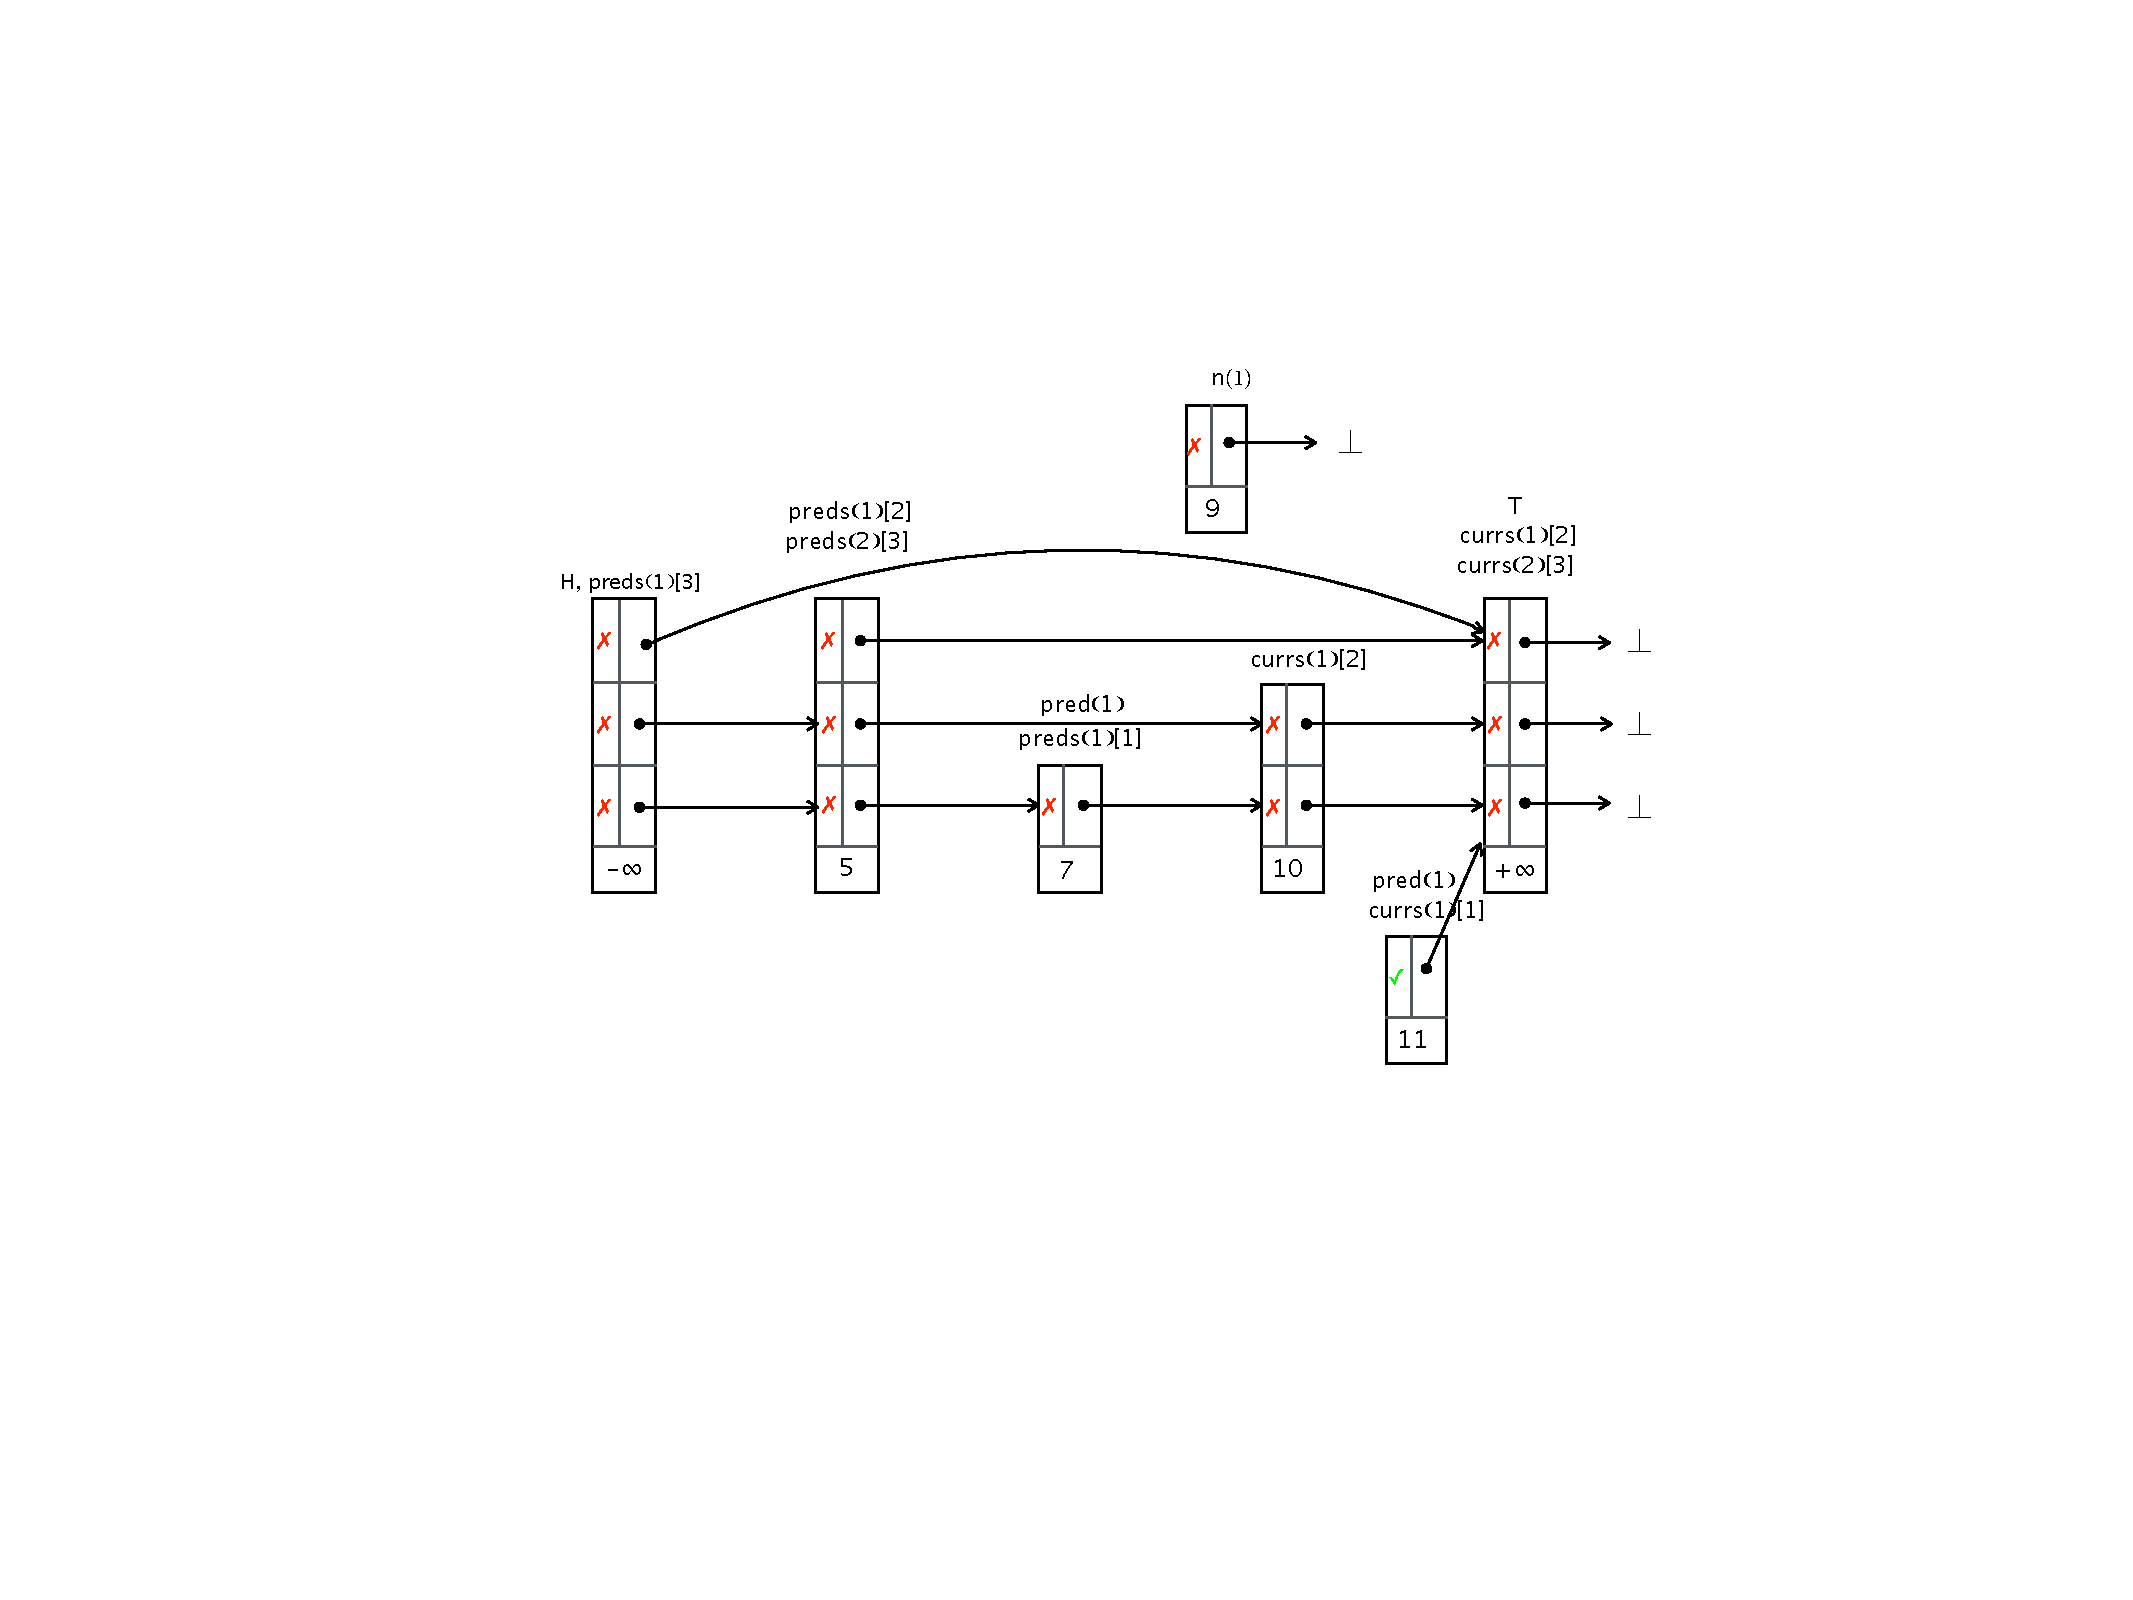
\includegraphics[width=1.2\textwidth, trim={7cm 8cm 0.5cm 6cm}, clip]{skipshape.pdf}  
 \caption{A concrete shape of 3-level skiplist}
\label{sl-shape}
\end{figure}

%\todo[inline]{Quy: you must provide example heaps, etc. before I can continue
%  writing}
Figure~\ref{sl-shape} shows an example heap state of the
skiplist algorithm with three levels. Each heap cell is shown with the values of its {\tt mark} and {\tt key} fields. %\bjcom{Add a legend, showing the layout of fields, as in previous papers}
Let us illustrate how pairs of heap nodes can be represented by fragments.
Figure~\ref{fig:skiplistabs} shows a set of fragments that is sufficient to
represents the configuration in Figure~\ref{sl-shape}. There are $11$ fragments, named $\frag_1$, \ldots , $\frag_{11}$. Three of
these ($\frag_9$, $\frag_{10}$ and $\frag_{11}$) consist of a tag that points to $\dangconst$. All other fragments consist of a pair of pointer-connected tags. The fragments $\frag_1$, $\frag_2$,$\frag_3$,$\frag_4$,$\frag_5$,$\frag_9$ and $\frag_{10}$ are level-1-fragments, whereas the other fragments are higher level-fragments. The $\tt private$ field of the input tag of $\frag_7$ is $\tt true$, whereas the $\tt private$ field of other tags of other fragments are $\tt false$. The two left-most cells
in Figure~\ref{sl-shape} are represent by the level 1-fragment $\frag_1$ in
Figure~\ref{fig:skiplistabs}. Here, the variable $\tt preds[3]$ is represented by $\tt preds[higher]$. The mapping $\pi_1$ represents the data abstraction of the $\tt key$ field, here saying that it is smaller than the value $9$ of the observer register. Note that, in our approach, the data abstraction is a mapping function from data value to a set of observer registers.
The two left-most cells are also represented by
a higher-level fragment, viz.\ $v_6$.
The pair consisting of the two sentinel cells (with keys $\tt -\infty$ and $\tt +\infty$) are represented by the higher-level fragment $v_7$. In each fragment, the abstraction values of non-pointer fields are shown represented inside each tag of the fragment. The data relation is shown as a label on the  arrow between two tags. Above each tag is pointer variables. The first row under each tag is reach from information, whereas the second row is reach to information.
 \begin{figure}
\center
	\input skiplistabs
\caption{Fragment abstraction of skiplist algorithm}
\label{fig:skiplistabs}
\vspace*{-0.6cm}
\end{figure} 


\chapter{Related Work}
This chapter reviews related work, along the main topics of this thesis including: verification of linearizabilities of concurrent algorithms, 
sequential shape analysis and concurrent techniques.
\section{Verification of Linearizabilities}
There are several previous work on verification of linearizabilities of concurrent programs[9,12,13,34]. In which, verification of conformance to a simple abstract specification has been performed
using refinement techniques, which establish simulation relations between the implementation and specification, using
partly manual techniques. Vafeiadis \cite{Vafeiadis:Thesis}
uses forward and backward simulation relations together with history or prophecy variables to prove linearizability. These approaches are manual, and without tool implementations.
%Much previous work has been devoted to the {\it manual} verification of linearizability for concurrent programs such as \cite{Aaron:locigcal:linearizability}. 



{\it Mechanical} proofs of linearizability, using interactive theorem
provers, have been reported in 
\cite{Colvin:Lazy-List,Derrick:fm14,SWD:cav12,SDW:tcl14}.
%
For instance, Colvin {\it et al.} \cite{Colvin:Lazy-List}
verify the lazy set algorithm in  PVS,
using a combination of forward and backward simulations. In \cite{OHearnlist}, O'Hearn {\it et al.}  define a {\it hindsight lemma} that provides a non-constructive evidence for linearizability. The lemma assumes that the algorithm maintains certain simple invariants which are resilient to interference, and which
can themselves be verified using purely thread-local proofs. As a
consequence, the lemma allows us to unlock a perhaps-surprising
intuition: a high degree of interference makes non-trivial highly concurrent algorithms in some cases much easier to verify than less
concurrent ones.
The lemma is used to prove linearizability of an optimistic variant of 
the lazy set algorithm.
%%% AUTOMATED LINEARIZATION

There are several works on {\it automatic} verification of linearizability.
the works~\cite{AHHR:integrated,BLMRS:cav08,Vafeiadis:vmcai09}
all require fixed linearization points.
In \cite{Vafeiadis:cav10}, Vafeiadis
develops an automatic technique for proving  linearizability that
employs instrumentation to verify logically pure executions.
However, this work can handle non-fixed LPs only for read-only methods,
i.e, methods that do not modify the heap.
%
This means that the method cannot handle
 algorithms like the {\it Elimination} queue ~\cite{Shavit:ElimQueue}, {\it HSY} stack~\cite{HSYstack}, {\it CCAS}~\cite{Harris:CAS}, 
{\it RDCSS}~\cite{Harris:CAS} and {\it HM} set~\cite{ArtOfMpP} that we consider in the thesis. In addition, their shape abstraction is not powerful enough to handle algorithms like {\it Harris} set~\cite{Harris:list} and {\it Michael} set~\cite{Michael:list} that are also handled by technique in this thesis.
Chakraborty {\it et al.} \cite{HSV:concur13}
describe an ``aspect-oriented'' method for  modular verification 
of concurrent queues that they use to prove linearizability of the Herlihy/Wing queue.
Bouajjani et al. \cite{BEEH:icalp15} extended this work to show that verifying 
linearizability for certain
fixed abstract data types, including queues and stacks, is reducible to 
control-state reachability. 
%
We can incorporate this technique into
our framework by a suitable construction of observers.
The method can not be applied to sets.
%
  
%
Vechev {\it et al.}~\cite{Vechev:spin09}
check linearizability with user-specified non-fixed LPs,
using a tool for finite-state verification.
Their method assumes a bounded number of threads, and
they report state space explosion when having more than two threads.
%
Dragoi  {\it et al.} \cite{Henzinger:CAV13} describe a method for proving
linearizability that is applicable to algorithms with non-fixed LPs.
%
However, their method needs to rewrite the implementation so that all operations 
have linearization points within the rewritten code.
%
\v{C}ern{\'y} {\it et al} \cite{CernyRZCA:CAV10} show decidability of a class
of programs with a bounded number of threads operating on concurrent data structures.


The most recent work of Zhu {\it et al.} \cite{Poling}
describe a tool using {\it hindsight lemma} and SMT solver to proof linearizabilities, they can handle several specific set, queue, and stack  
algorithms. For queue algorithms, their technique can handle queues with helping mechanism except for {\it HW} queue~\cite{HeWi:linearizability} which is handled by this thesis.
%
For set algorithms, the authors can only handle those that perform an optimistic contains (or lookup) operation by applying the {\it hindsight lemma} from 
\cite{OHearnlist}. 
%
Hindsight-based proofs provide only {\it non-constructive} 
evidence of linearizability. Algorithms with non-optimistic contains (or lookup) operation like {\it HM}~\cite{ArtOfMpP}, {\it Harris}~\cite{Harris:list} and {\it Michael}~\cite{Michael:list} sets cannot be verified by their technique.


We have not found any report in the literature of a
verification method that is sufficiently powerful to
automatically verify the class of concurrent set
implementations based or sorted and non-sorted
singly-linked lists having non-optimistic contains (or lookup) operations we consider. For instance %For instance,
%the shape abstraction of the CAVE implementation
%\cite{Vafeiadis:cav10}
%is not powerful enough to handle
the lock-free sets of {\it HM}~\cite{ArtOfMpP},
{\it Harris}~\cite{Harris:list}, or {\it Michael}~\cite{Michael:list},
or unordered set of~\cite{Zhang:unorderedlist},
%reported in
%Section~\ref{section:experiments} (as also confirmed by the CAVE
%tool implementors).
%The same applies to
%the tool in~\cite{Poling}.


\section{Shape Analysis}
\subsection{Sequential Shape Analysis}
Our approach builds on the fully automated FA-based
approach for shape analysis of programs with complex dynamic linked data
structures \cite{forester11,Forester}. We significantly extend this approach by
allowing it to track ordering relations between data values stored inside
dynamic linked data structures. 

For shape analysis, many other formalisms than FA have been used, including,
e.g., separation logic and various related graph formalisms
\cite{Hongseok:SL,thor10,rival11,Kamil:SL}, other logics \cite{SagivRW02,Jakob:ML},
automata \cite{artmc12}, or graph grammars \cite{Jonathan:Shape}. Compared with FA,
these approaches typically handle less general heap structures (often restricted
to various classes of lists) \cite{Hongseok:SL,Kamil:SL}, they are less
automated (requiring the user to specify loop invariants or at least inductive
definitions of the involved data structures)
\cite{thor10,rival11,Kamil:SL,Jonathan:Shape}, or less scalable \cite{artmc12}.

Verification of properties depending on the ordering of data stored in SLLs was
considered in~\cite{lists-counters}, which translates programs with SLLs to
counter automata. A subsequent analysis of these automata allows one to prove
memory safety, sortedness, and termination for the original programs. The work
is, however, strongly limited to SLLs. In our technique, we get inspired by the way
that \cite{lists-counters} uses for dealing with ordering relations on data, but
we significantly redesign it to be able to track not only ordering between
simple list segments but rather general heap shapes described by FA. In order to
achieve this, we had to not only propose a suitable way of combining ordering
relations with FA, but we also had to significantly modify many of the
operations used over FA.

In~\cite{atva09}, another approach for verifying data-dependent properties of
programs with lists was proposed. However, even this approach is strongly
limited to SLLs, and it is also much less efficient than our current approach.

%In~\cite{AHHR:integrated:rep}, concurrent programs operating on SLLs are analyzed
%using an adaptation of a transitive closure logic~\cite{BiRa:vmcai06}, which
%also tracks simple sortedness properties between data elements.

Verification of properties of programs depending on the data stored in dynamic
linked data structures was considered in the context of the TVLA tool
\cite{Loginov:AbstrRefViaInductLearning:05} as well. Unlike our approach,
\cite{Loginov:AbstrRefViaInductLearning:05} assumes a fixed set of shape
predicates and uses inductive logic programming to learn predicates needed for
tracking non-pointer data. The experiments presttented in
\cite{Loginov:AbstrRefViaInductLearning:05} involve verification of sorting and
stability properties of several programs on SLLs (merging, reversal,
bubble-sort, insert-sort) as well as insertion and deletion in BSTs. We do not
handle stability, but for the other properties, our approach is much faster.
Moreover, for BSTs, we verify that a node is greater/smaller than all the nodes
in its left/right subtrees (not just than the immediate successors as in
\cite{Loginov:AbstrRefViaInductLearning:05}).

An approach based on separation logic extended with constraints on the data
stored inside dynamic linked data structures and capable of handling size,
ordering, as well as bag properties was presented in \cite{rival11}. Using the
approach, various programs with SLLs, DLLs, and also AVL trees and red-black
trees were verified. The approach, however, requires the user to manually
provide inductive shape predicates as well as loop invariants.  Later, the need
to provide loop invariants was avoided in \cite{sleek13}, but a need to manually
provide inductive shape predicates remains.

Another work that targets verification of programs with dynamic linked data
structures, including properties depending on the data stored in them, is
\cite{Hongseok:SL}. It generates verification conditions in an undecidable
fragment of higher-order logic and discharges them using decision procedures,
first-order theorem proving, and interactive theorem proving. To generate the
verification conditions, loop invariants are needed. These can either be
provided manually or sometimes synthesized semi-automatically using the approach
of \cite{SagivRW02}. The latter approach was successfully applied to several
programs with SLLs, DLLs, trees, trees with parent pointers, and 2-level skip
lists. However, for some of them, the user still had to provide some of the
needed abstraction predicates.
Several works, including~\cite{dragoi:atva12}, define frameworks for reasoning
about pre- and post-conditions of programs with SLLs and data. Decidable
fragments, which can express more complex properties on data than we consider,
are identified, but the approach does not perform fully automated verification,
only checking of pre-post condition pairs.


\subsection{Concurrent Shape Analysis}
There are several approaches for automated verification of concurrent algorithms are limited to the
case of singly-linked
lists~\cite{AHHR:integrated,meyer:vmcai16,Quy:sas16,Sagiv:correlation,Vafeiadis:cav10}.
Furthermore, many of these techniques impose additional restrictions on the considered verification problem, such as bounding the number of accessing
threads~\cite{Amit:comparisonAbstraction,Vechev:spin09,CernyRZCA:CAV10}.

In~\cite{AHHR:integrated}, concurrent programs operating on SLLs are analyzed
using an adaptation of a transitive closure logic~\cite{BiRa:vmcai06}, combined with
tracking of simple sortedness properties between data elements; the approach does
not allow to represent patterns observed by threads when following sequences of
pointers inside the heap, and so has not been applied to concurrent set
implementations.
In our recent work~\cite{Quy:sas16}, we extended this approach to handle SLL implementations
of concurrent sets by adapting a
well-known abstraction of singly-linked lists ~\cite{MYRS:Canonical} for concurrent programs.
The resulting technique is specifically tailored for singly-links.
Our fragment abstraction is significantly simpler conceptually, and can therefore be  adapted
also for other classes of heap structures.
The approach of~\cite{Quy:sas16} is the only one with a shape representation strong enough to
verify  concurrent set
implementations based on sorted and non-sorted
singly-linked lists having non-optimistic contains (or lookup) operations we consider, such as
the lock-free sets of {\it HM}~\cite{ArtOfMpP},
{\it Harris}~\cite{Harris:list}, or {\it Michael}~\cite{Michael:list},
or unordered set of~\cite{Zhang:unorderedlist}. Our fragment abstraction can handle them
as well as also algorithms employing skiplists and arrays of singly-linked lists.

There is no previous work on automated verification of skiplist-based concurrent algorithms. The work~\cite{Sanchez:skiplists}
generates verification conditions for statements in sequential skiplist implementations. All these
works assume that skiplists have the well-formedness property that any higher-level lists is a
sublist of any lower-level list, which is true for sequential skiplist algorithms, but false for
several concurrent ones, such as~\cite{ArtOfMpP,Linden:opodis13}.



Concurrent algorithms based on arrays of SLLs, and including timestamps, e.g.,
for verifying the algorithms in~\cite{ts-stack} have shown to be rather challenging. Only
recently has the TS stack been verified by non-automated
techniques~\cite{BEEM:cav17} using a non-trivial extension of
forward simulation, and the TS queue been verified manually by a new technique
based on partial orders~\cite{Khyzha:esop17,singh:issre16}..
We have verified both these algorithms automatically using fragment abstraction,

Our fragment abstraction is related in spirit to other formalisms that
abstract dynamic graph structures by defining some form of equivalence on
its nodes (e.g.,~\cite{spotlight07,SagivRW02}). These have
been applied to verify functional correctness fine-grained concurrent
algorithms for a limited number of SLL-based algorithms. Fragment
abstraction's representation of both local and global information allows to
extend the applicability of this class of techniques.



